\documentclass[12pt]{article}

\usepackage[section]{placeins}
\usepackage[font={small,it}]{caption}
\usepackage[% 
                  bookmarks,% 
                  bookmarksopen=false,% Klappt die Bookmarks in Acrobat aus 
                  pdfauthor={Tom Schöner},% 
                  pdftitle={TFP Evaluation},% 
                  colorlinks=true,% 
                  linkcolor=blue,% 
                  citecolor=red,%
                ]{hyperref}
\usepackage{multicol}
\usepackage{lingmacros}
\usepackage{tree-dvips}
\usepackage{graphicx}
\usepackage{amsmath}
\usepackage{amssymb}
\usepackage{siunitx}
\usepackage{ngerman}

\usepackage{xparse}

\usepackage[utf8]{inputenc}
\usepackage{siunitx}
\usepackage[numbers]{natbib} % omit 'round' option if you prefer square brackets
\usepackage{wrapfig}

\usepackage{microtype}% verbesserter Randausgleich

\usepackage{titlesec}


\usepackage{listings}

\usepackage{color}
 
\definecolor{codegreen}{rgb}{0,0.6,0}
\definecolor{codegray}{rgb}{0.5,0.5,0.5}
\definecolor{codepurple}{rgb}{0.58,0,0.82}
\definecolor{backcolour}{rgb}{0.99,0.99,0.99}

\lstdefinestyle{mystyle}{
    backgroundcolor=\color{backcolour},   
    commentstyle=\color{codegreen},
    keywordstyle=\color{magenta},
    numberstyle=\tiny\color{codegray},
    stringstyle=\color{codepurple},
    basicstyle=\scriptsize,
    breakatwhitespace=false,         
    breaklines=true,                 
    captionpos=b,                    
    keepspaces=true,                 
    numbers=left,                    
    numbersep=5pt,                  
    showspaces=false,                
    showstringspaces=false,
    showtabs=false,                  
    tabsize=2
}

 
\lstset{style=mystyle}

\titleformat{\section}
   {\normalfont\Large\bfseries\raggedright}{\thesection}{1em}{}
\titleformat{\subsection}
   {\normalfont\large\bfseries\raggedright}{\thesubsection}{0.8em}{}

\hypersetup{pageanchor=false}
\linespread{1.15}

\renewenvironment{quote}{%
   \list{}{%
     \leftmargin0.3cm   % this is the adjusting screw
     \rightmargin\leftmargin
   }
   \item\relax
}
{\endlist}

\bibliographystyle{plainnat}

%----------------------------------------------------------------------------------------

\begin{document}
\begin{titlepage}

\newcommand{\HRule}{\rule{\linewidth}{0.5mm}} % Defines a new command for the horizontal lines, change thickness here

\begin{center}
 
%----------------------------------------------------------------------------------------
%	HEADING SECTIONS
%----------------------------------------------------------------------------------------

\textsc{\LARGE HAW Hamburg}\\[0.5cm] % Name of your university/college
\textsc{\LARGE Informatik Master}\\[1.5cm] % Name of your university/college
\textsc{\Large Grundprojekt}\\[0.5cm] % Major heading such as course name

%----------------------------------------------------------------------------------------
%	TITLE SECTION
%----------------------------------------------------------------------------------------

\HRule \\[0.4cm]

{ \large \bfseries Evaluation of TensorFlow Probability}\\[0.1cm]
{ \large for enhanced machine learning}\\[0cm]

\HRule \\[2.0cm]

%----------------------------------------------------------------------------------------
%	AUTHOR SECTION
%----------------------------------------------------------------------------------------

\begin{minipage}{\textwidth}
\begin{flushleft} \large
\emph{Bearbeiter:}\\
Tom Schöner (2182801) \linebreak
\end{flushleft}
\end{minipage}
~
\begin{minipage}{\textwidth}
\begin{flushleft} \large
\emph{Betreuung:} \\
Prof. Dr. Olaf Zukunft
\end{flushleft}
\end{minipage}\\[4cm]

%----------------------------------------------------------------------------------------
%	DATE SECTION
%----------------------------------------------------------------------------------------

\vspace{\fill} % Fill the rest of the page with whitespace

{\large \today}\\[3cm] % Date, change the \today to a set date if you want to be precise

\end{center}

\end{titlepage}


%----------------------------------------------------------------------------------------

\tableofcontents

\newpage

%----------------------------------------------------------------------------------------
%	Content
%----------------------------------------------------------------------------------------

\section{Abstract}
\label{abstract}
Die auf Tensorflow basierende Bibliothek Tensorflow Probability\footnote{\url{https://www.tensorflow.org/probability}} v0.7.0 --- fortan mit \textit{TFP} abgekürzt --- erweitert das Framework um eine probabilistische Komponente.
Mittels einer breiten Masse an bereitgestellten Tools, wie statistischen Verteilungen, Sampling oder verschiedenster probabilistischer Funktionen für neronale Netze, können einfache bis hin zu komplexen Modellen erstellt werden. Berechnungen werden, wie man es aus Tensorflow gewohnt ist, durch \textit{Dataflow Graphs}\footnote{\url{https://www.tensorflow.org/guide/graphs}} abgebildet. Auf die verschiedenen Funktionsweisen und Schichten von TFP wird in Abschnitt \ref{sec:tfp-components} detaillierter eingegangen.

In dieser Evaluation soll die Bibliothek auf ihre Semantik, Effektivität beim Erstellen von statistischen Modellen und Integration in das Framework Tensorflow untersucht werden. Das maschinelle Lernen mit Hilfe von neuronalen Netzen und deren Abstraktion durch Keras ist hierbei als Schwerpunkt anzusehen.

\section{Tensorflow Probability Komponenten}
\label{sec:tfp-components}
Die Struktur von TFP lässt sich, wie aus der Dokumentation zu entnehmen ist\footnote{\url{https://www.tensorflow.org/probability/overview}}, in die folgenden vier Schichten einteilen. Die Schichten bauen hierarchisch aufeinander auf, abstrahieren die unterliegenden Schichten aber nicht zwangsläufig. Möchte man beispielsweise durch \textit{MCMC} in Schicht 3 Parameter seines probabilistischen Modells mittels Sampling ermitteln, sollten \textit{Bijectors} aus Schicht 1 kein Fremdwort sein.

\subsection{Schicht 0: Tensorflow}
TFP ist nicht als eigenständige Komponente neben Tensorflow anzusehen, sondern als Bestandteil dessen. Die probabilistischen Berechnungen werden innerhalb von Tensorflow Sessions oder im \textit{Eager}-Modus ausgeführt. Tensorflow wird von mehreren Programmiersprachen wie Python, JavaScript oder C++ unterstützt. Die Bibliothek TFP ist aktuell nur für die primär unterstützte Programmiersprache Python implementiert.

\subsection{Schicht 1: Statistical Building Blocks}
\label{sec:buildingblocks}
Als Fundament statistischer Modelle sind mehrere, in Python Module aufgeteilte, Klassen und Funktionen gegeben. Diese können in der API Dokumentation der TFP Website eingesehen werden. Ein Beispiel hierfür ist das Modul \textbf{fp.stats}. Unter \textbf{fp.stats} finden sich unter Anderem Funktionen für die Berechnung für Korrelationen, Quantilen oder Standardabweichungen. Diese Funktionen sind auf die Verwendung von Tensoren ausgelegt, lassen sich aber generell auch mit normalen n-dimensionalen Python Arrays oder Numpy Arrays aufrufen.  

Verschiedenste, für probabilistische Modelle essentielle Verteilungen reihen sich unter dem Modul \textbf{tfp.distributions} in dieser Schicht ein: \textit{Normal-, Bernoulli-, Exponential- oder Gammaverteilung}, um einige zu nennen. Generell erben Klassen für Verteilungen, wie etwa die Normalverteilung, von der Klasse \textbf{tfp.distributions.Distribution}\footnote{\url{https://www.tensorflow.org/probability/api_docs/python/tfp/distributions/Distribution}}. Diese gemeinsame Schnittstelle standardisiert die Benutzung. Sie fordert zudem Implementationen mehrerer hilfreicher Methoden wie etwa für die logarithmische Wahrscheinlichkeit oder dem Mittelwert. Am Beispiel der Normalverteilung mit der Definition $X \sim \mathcal{N}(\mu,\,\sigma^{2})$ sind im Folgenden einige der Funktionen aufgeführt (siehe Listing \ref{lst:normal}). Visualisiert man die Verteilung auf Basis der Samples \textit{sample} (Zeile 4) ergibt sich Abbildung \ref{fig:normal_dist}.

\begin{lstlisting}[language=Python, caption={Verwendung der Klasse tfp.distributions.Normal}, label={lst:normal}]
normal_dist = tfd.Normal(name="N", loc=0., scale=1.)
# tfp.distributions.Normal("N/", batch_shape=(), event_shape=(), dtype=float32)

sample = normal_dist.sample(sample_shape=25000)
# <tf.Tensor: id=188, shape=(25000,), dtype=float32, numpy=array([-0.45733708, -0.19126031, -0.33290815, ..., -1.1285563 , -0.6958163 ,  0.552399  ], dtype=float32)>

normal_dist.mean() 
# tf.Tensor(0.0, shape=(), dtype=float32)

normal_dist.prob(1.0) 
# tf.Tensor(0.24197072, shape=(), dtype=float32)
\end{lstlisting}


\begin{figure}[h]
    \centering
    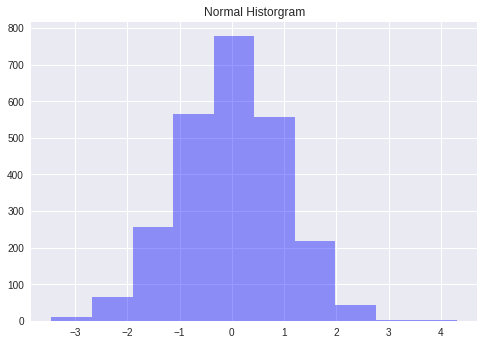
\includegraphics[width=0.8\textwidth]{./figs/normal-dist.png}
    \caption{$X \sim \mathcal{N}(0,\, 1)$ mit 25000 Samples}
    \label{fig:normal_dist}
\end{figure}

% Shapes
\textit{Broadcasting, batching} und \textit{shapes} sorgen dafür, dass unabhängige Verteilungen als sogenannter Batch in einer Entität  gekapselt werden können. Um beispielsweise ein zweidimensionales Batch für die Normalverteilung aus Listing \ref{lst:normal} zu erzeugen, kann als Erwartungswert $\mu$ \textit{loc=[0., 10.]} übergeben werden. TFP unterstützt broadcasting, somit müssen die folgenden Aufrufe nicht angepasst werden. Das Ergebnis wird ebenfalls Zweidimensional sein. Broadcasting verhält sich analog zu dem in Numpy etablierten Konzept\footnote{\url{https://docs.scipy.org/doc/numpy/user/basics.broadcasting.html}}.

Die Shapes lassen sich nochmals in drei Kategorien unterteilen, Tabelle \ref{table:shapes} verdeutlicht diese an einem Beispiel.
\begin{itemize}
  \item \textit{event shape}: Beschreibt die Form einer Stichprobe aus einer Verteilung, abhängig von seiner Dimension. Skalare Verteilungen besitzen die Form [], multivariate Verteilungen zum Beispiel die Form [3].
  \item \textit{batch shape}: Beschreibt die Form unabhängiger, nicht identisch verteilter Stichproben.
  \item \textit{sample shape}: Beschreibt die Form unabhängiger, aber identisch verteilter Stichproben aus \textit{batches} der Verteilung(en).
\end{itemize}

\begin{table}[]
\centering
\begin{tabular}{|l|l|}
\hline
sample shape  & Ergebnis        \\ \hline
1             & (1, 2, 3)       \\ \hline
2             & (2, 2, 3)       \\ \hline
{[}1, 5{]}    & (1, 5, 2, 3)    \\ \hline
{[}3, 4, 5{]} & (3, 4, 5, 2, 3) \\ \hline
\end{tabular}
\caption{Auswirkung der verschiedenen sample shapes mit einem batch shape von [2] und einem event shape von [3]}
\label{table:shapes}
\end{table}


Ein weiterer Bestandteil von Schicht 1 sind \textit{Bijectors}. Bijectors bilden eine Zahl aus $\mathbb{R}^n$ auf $\mathbb{R}^m$ ab oder jeweils einer Submenge dieser. Aufgrund der im Bijector hinterlegten bijektiven Funktion ist dieser Schritt umkehrbar, daher: $x = f^{-1}(f(x))$. Dies ist besonders bei der Transformierung von Stichproben aus Verteilungen nützlich und wird folglich für das Erstellen von Modellen (Abschnitt \ref{sec:layer2}) und Berechnungen probabilistischer Interferenzen (Abschnitt \ref{sec:layer3}) eingesetzt. TFP bietet bereits einige vorgefertigte Bijectors unter \textbf{tfp.bijectors}\footnote{\url{https://www.tensorflow.org/probability/api_docs/python/tfp/bijectors}} an. 


\subsection{Schicht 2: Model Building}
\label{sec:layer2}

% Probabilistic Layers (with Keras)
Keras ist eine modulare high-level API für die Erstellung und Komposition neuronaler Netze. TFP erweitert das Angebot an Keras-kompatiblen Komponenten durch einige probabilistische Schichten in \textbf{tfp.layers}. Die Architektur orientiert sich weiterhin am selben Keras Model\footnote{\url{https://keras.io/getting-started/sequential-model-guide/}}. Neben vorgefertigten Schichten wie \textbf{tfp.layers.IndependentNormal} lassen sich durch die Klasse \textbf{tfp.layers.DistributionLambda} alle Verteilungen, welche von \textbf{tfp.distributions.Distribution} erben, in die Sequenz einbinden. Keras für Tensorflow erlaubt nur konkrete Tensoren und keine generischen Verteilungen, daher muss   die jeweilige Schicht wissen, wie sie ihren Ausgabevektor definieren soll. Dies geschieht mittels des übergebenen Parameters \textit{convert\_to\_tensor\_fn}, welcher standardmäßig durch die \textit{sample} Funktion repräsentiert wird. Hierdurch ist eine konfigurierbare Transformation in einen konkreten Tensor gewährleistet.

Die Einbindung von probabilistischen Schichten in Keras ist Anfangs noch ungewohnt, da sie nicht ganz der herkömmlichen Herangehensweise entspricht. Für ein funktionierendes Modell müssen die internen Ein- und Ausgabevektors untereinander Kompatibel sein. Sobald das Modell mit \textit{compile()} und \textit{train()} kompiliert und trainiert wurde, können Prognosen mit neuen Daten vorgenommen werden. Die Prognose liefert praktischer Weise direkt eine Wahrscheinlichkeitsverteilung zurück, dessen batch shape (siehe Abschnitt \ref{sec:buildingblocks}) an die Form der neuen Daten angepasst ist. Haben die neuen Daten die Form [100], so ergibt sich für die Verteilung beispielsweise ein batch shape von [100, 1] und repräsentiert somit 100 unabhängige, nicht zwangsläufig gleich verteilte Stichproben. Die über das Training ermittelten Gewichte der Eingabevektoren solcher probabilistischen Schichten lassen sich als Parameter der Verteilung interpretieren, natürlich abhängig von der genauen Implementierung.

Die Interpretation der Gewichte sowie die Verwendung und der Umgang mit Ein- und Ausgabevektoren von probabilistischen Schichten in Keras wird in Abschnitt \ref{sec:example_air_quality} anhand eines Beispiels verdeutlicht. Listing \ref{lst:tfp.layers.IndependentNormal} zeigt die Verwendung von verschiedenen probabilistischen und nicht probabilistischen Keras Schichten. Das Beispiel ist der Dokumentation\footnote{\url{https://www.tensorflow.org/probability/api_docs/python/tfp/layers/IndependentNormal}} entnommen. 

\begin{lstlisting}[language=Python, caption={Beispiel probabilistischer und nicht probabilistischer Keras Schichten}, label={lst:tfp.layers.IndependentNormal}]
tfd = tfp.distributions
tfpl = tfp.layers
tfk = tf.keras
tfkl = tf.keras.layers

# Create a stochastic encoder - e.g., for use in a variational auto-encoder
input_shape = [28, 28, 1]
encoded_shape = 2
encoder = tfk.Sequential([
  tfkl.InputLayer(input_shape=input_shape),
  tfkl.Flatten(),
  tfkl.Dense(10, activation='relu'),
  tfkl.Dense(tfpl.IndependentNormal.params_size(encoded_shape)),
  tfpl.IndependentNormal(encoded_shape)
])
\end{lstlisting}

% Edward
Ein weiterer Bestandteil ist die probabilistische Programmiersprache Edward2\footnote{\url{https://github.com/tensorflow/probability/tree/master/tensorflow_probability/python/edward2}}.

\subsection{Schicht 3: Probabilistic Inference}
\label{sec:layer3}
Als letzte Schicht enthält TFP Werkzeuge für probabilistische Inferenz. Dazu gehören \textit{Marcov chain Monte Carlo (MCMC)} Algorithmen, \textit{Variational Inference} Algorithmen und stochastische Optimierungsverfahren. 

Durch Sampling ermöglicht MCMC das Berechnen statistischer Modelle mit einer hohen Anzahl an Parametern. Eine analytische Herangehensweise ist bereits ab wenigen Parametern nicht mehr sinnvoll, da hierfür die Bestimmung eines multidimensionalen Integrals erforderlich wäre. TFP bietet mehrere MCMC Algorithmen unter \textbf{tfp.mcmc} an. 

Listing \ref{lst:mcmc} zeigt einen Ausschnitt der Verwendung des Hamiltonian Monte Carlo Algorithmus. Die hier nicht enthaltene Auswertung würde in einer approximierten Verteilung des Parameters \textit{tau} für das gegebene Modell \textit{\_data\_model} resultieren. Ein praxisbezogenes und ausführlicheres Beispiel ist unter \url{https://github.com/tom-schoener/ml-probability/blob/master/tfp-evaluation/notebooks/mcmc.ipynb} einsehbar.

\begin{lstlisting}[language=Python, caption={Verwendung des Hamiltonian Monte Carlo Algorithmus (gekürzt)}, label={lst:mcmc}]
# Set the chain's start state.
initial_chain_state = [ 0.5 * tf.ones([], dtype=tf.float32, name="init_tau") ]

def joint_log_prob(_data_model, tau):
  rv_tau = tfd.Uniform()
  rv_observation = tfd.Poisson(rate=rv_tau)

  return rv_tau.log_prob(tau) + tf.reduce_sum(rv_observation.log_prob(_data_model))

# setup the chain
[ tau ], kernel_results = tfp.mcmc.sample_chain(
  num_results=1000,
  num_burnin_steps=500,
  current_state=initial_chain_state,
  kernel=tfp.mcmc.TransformedTransitionKernel(
    inner_kernel=tfp.mcmc.HamiltonianMonteCarlo(
      target_log_prob_fn=lambda tau: joint_log_prob(_data_model, tau)),
    bijector=[ tfp.bijectors.Sigmoid() ] # Maps [0,1] to R  
  )
)
\end{lstlisting}

Die in der API verwendeten Bezeichnungen decken sich hier größtenteils mit der in der Literatur verwendeten Sprache, wodurch sich Methoden anderer Quellen relativ problemlos übertragen lassen. 

Zu den Optimierungsverfahren von TFP gehören verschiedenste Algorithmen. Ohne an dieser Stelle zu sehr ins Detail zu gehen, gibt es beispielsweise unter \textbf{tfp.optimizer.bfgs\_minimize}\footnote{\url{https://www.tensorflow.org/probability/api_docs/python/tfp/optimizer/bfgs_minimize}} einen \textit{Optimzer}\cite{Nocedal2006}, welcher einen Tiefpunkt einer differenzierbaren Funktion approximiert ermittelt. Vergleichbar sind diese Algorithmen mit dem bereits in Tensorflow enthaltenen Optimierungsverfahren\footnote{\url{https://www.tensorflow.org/versions/r2.0/api_docs/python/tf/optimizers}}.

\textit{Variational Inference} in TFP habe ich für diese Evaluation nicht weiter untersucht.

\section{Semantik und Projektarchitektur}

\subsection{Fehlerbehandlung}
Ein nicht zu vernachlässigender Teil der Softwareentwicklung ist das Erkennen, Interpretieren und Beheben von semantischen Fehlern. Als Teil von Tensorflow gibt TFP bereits sinnvolle und leserliche Fehlermeldungen aus. Zum Beispiel wird bei falschen Typen eines Tensors folgende Fehlermeldung mit Stacktrace zurückgegeben: \textit{ValueError: Can't convert Python sequence with mixed types to Tensor}. Auf fehlende, nicht optionale Parameter wird ebenfalls hingewiesen. Befindet man sich nicht im Eager-Execution Modus, findet bereits beim Erstellen des Graphen und somit vor dessen Evaluation ein solches Typechecking statt. 

\subsection{Dokumentation}
TFPs offizielle Dokumentation bietet neben der Beschreibung der API eine Auflistung an Beispielen und weiterführenden Ressourcen. Die als Einführung anzusehende und kürzlich nach TFP portierte Version von \textit{Bayesian Methods for Hackers: Probabilistic Programming and Bayesian Inference}\cite{Davidson-Pilon2015} stellte sich als besonders Hilfreich heraus.

Die Bibliothek befindet sich in einem vergleichsweise frühen Stadium der Entwicklung. Es wird darauf hingewiesen, dass es in Zukunft zu Änderungen kommen kann. Teile der API sind entsprechend noch nicht vollständig dokumentiert (Stand März 2019).
Undokumentierte Funktionen sind allerdings eher die Ausnahme als die Norm. Ein Großteil der in dieser Evaluation verwendeten Schnittstellen ließ sich anhand von Beispielen, genaueren Erläuterungen der Parameter oder durch Verweise auf relevante Literatur und Paper nachvollziehen. Einzig ein Überblick oder eine Einleitung der individuellen Module und deren Funktionsweise fehlt fast vollständig. Die Verwendung dieser Module wird dadurch nicht sofort ersichtlich und erschwert deren Benutzung. Häufig musste ich auf Beispiele oder externe Quellen zurückgreifen, um mir einen Überblick zu verschaffen.

\section{Anwendungsgebiete}

Das Ziel maschinellen Lernens ist das Erkennen und Übertragen von Mustern. Reale Daten bringen allerdings immer eine gewisse Unsicherheit mit sich. Die Wahrscheinlichkeitstheorie wirkt diesem Problem, unter Anderem mit Hilfe der bayesschen Inferenz, entgegen. Prognosen lassen sich in Folge dessen auf mathematischer Grundlage einschätzen und verifizieren. Auch die (Hyper-)Parameter des Modells können als Zufallsvariable einer Wahrscheinlichkeitsverteilung dargestellt werden. Der probabilistische Ansatz schränkt die Anwendungsgebiete nicht ein, sondern bietet lediglich eine neue Sichtweise. Das folgende Beispiel soll diesen Vorteil und die Anwendung von TFP für probabilistische Modelle zeigen. In \textit{Machine Learning: A Probabilistic Perspective}\cite{Murphy2012} Kapitel 1.2.1.2 ff. (\textit{The need for probabilistic predictions}) werden weitere konkrete Beispiele wie die Klassifizierung von Blumen erläutert. 

\subsection{Beispiel: Korrelation von Luftverschmutzung und Temperatur}
\label{sec:example_air_quality}

Das Jupyter Notebook für das folgende Beispiel ist unter \url{https://github.com/tom-schoener/ml-probability/blob/master/tfp-evaluation/notebooks/air_quality.ipynb} einsehbar. Die Daten stammen aus dem \textit{UC Irvine Machine Learning Repository}\footnote{\url{https://archive.ics.uci.edu/ml/datasets/Air+quality}}.

Von März 2004 bis Februar 2005 wurden in einer italienischen Stadt nahe einer stark befahrenen Straße verschiedene Wetterdaten wie Temperatur, Luftfeuchtigkeit oder auch Stickstoffdioxidgehalt ($NO_2$) in der Luft stündlich gemessen. Die Daten für Temperatur, relativer Luftfeuchtigkeit und $NO_2$ sind aggregiert in den Abbildungen \ref{fig:temp}, \ref{fig:rh} und \ref{fig:no2} visualisiert. Die blaue Linie stellt den gemittelten Wert um 00:00Uhr Nachts und die orangene Linie um 12:00Uhr Mittags dar.

\begin{figure}[h]
    \centering
    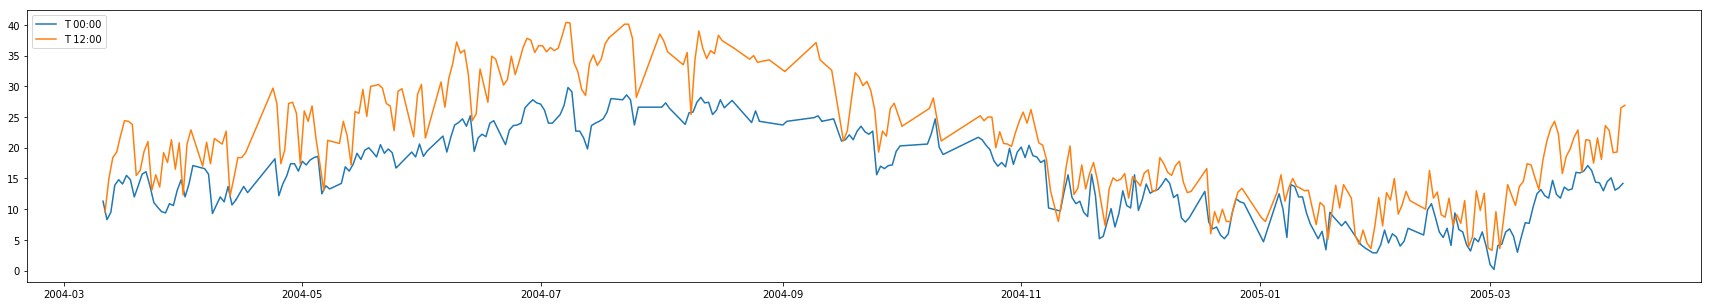
\includegraphics[width=1.0\textwidth]{./figs/temp.png}
    \caption{Temperatur in $^\circ\text{C}$}
    \label{fig:temp}
\end{figure}

\begin{figure}[h]
    \centering
    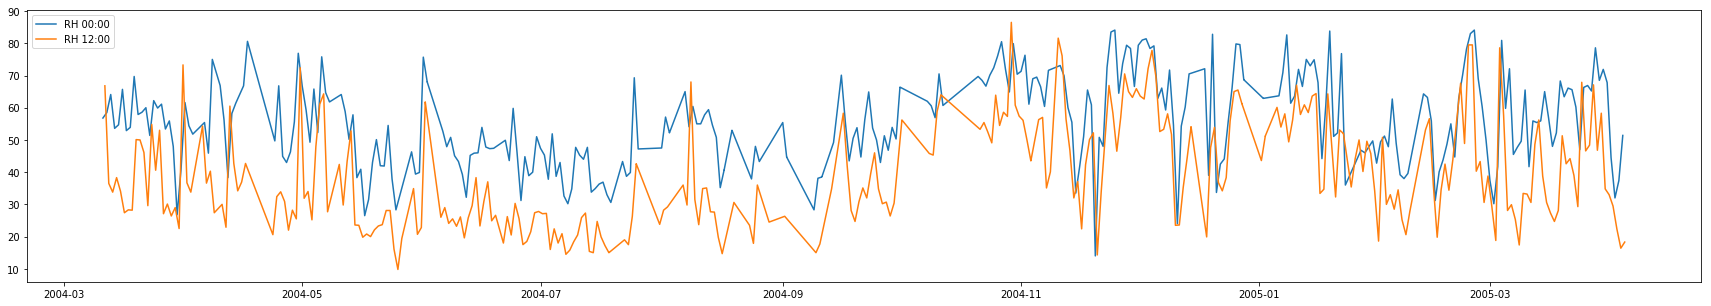
\includegraphics[width=1.0\textwidth]{./figs/rh.png}
    \caption{Relative Luftfeuchtigkeit in \%}
    \label{fig:rh}
\end{figure}

\begin{figure}[h]
    \centering
    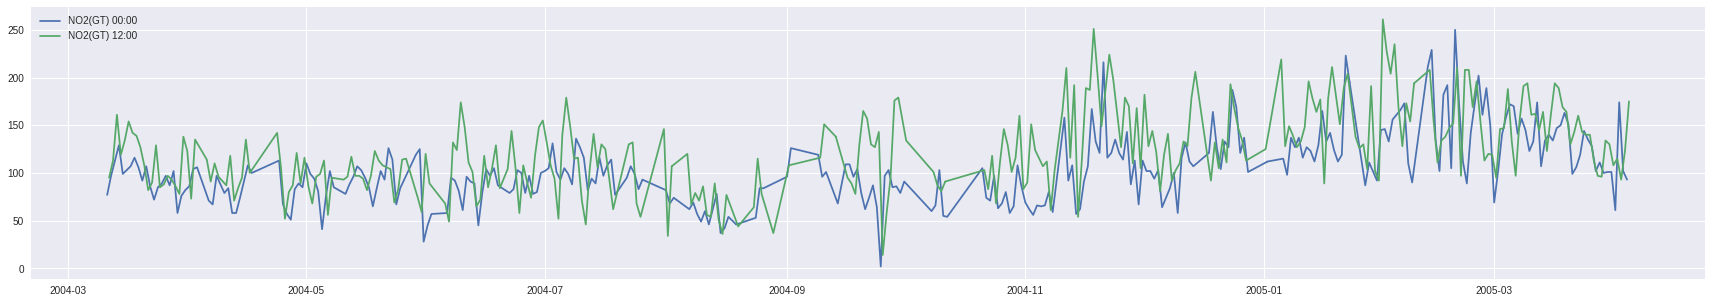
\includegraphics[width=1.0\textwidth]{./figs/no2.png}
    \caption{Stickstoffdioxid $NO_2$ in ${\mu g/m^3}$}
    \label{fig:no2}
\end{figure}

In Europa ist der Grenzwert von $NO_2$ gesetzlich auf max $200{\mu g/m^3}$ festgelegt. Die EU-Richtlinie 2008/50/EG verschärfte dieses Gesetz insofern, dass das Jahresmittel $40{\mu g/m^3}$ nicht überschreiten darf. In diesem Beispiel soll ein probabilistisches Modell für Aussagen über die Korrelation zwischen Temperatur und Luftverschmutzung auf Basis eines neuronalen Netzes in TFP erstellt werden. Da bei probabilistischen Modellen Verlust (\textit{loss}) mitmodelliert werden kann, wird nicht nur die Relation der Daten, sondern auch die Aussagekraft des jeweiligen ermittelten Wertes, zum Beispiel über dessen Standardabweichung, verdeutlicht.

\subsubsection{Modellierung ohne Unsicherheit}
\label{sec:no_unc}

Um das Modell erstellen zu können, müssen die Daten zunächst bereinigt werden. Null- oder fehlende Werte werden der Einfachheit halber interpoliert. In Listing \ref{lst:model_no_uncertainty} ist das Erstellen eines einfachen linearen Modells mit TFP und Keras zu sehen. Das Modell besteht aus zwei Schichten: Einem \textit{dense layer} mit einem eindimensionalen Ausgabevektor und eine durch eine Normalverteilung beschriebene Schicht, deren Input-Vektor durch den Ausgabevektor des \textit{dense layers} befüllt wird. Die Normalverteilung benutzt seinen Input, um den Mittelwert zu bestimmen. Beim Trainieren des Modells wird der Verlust (\textit{loss}) durch die Funktion \textit{neg\_log\_lik}, daher dem negativen Logarithmus einer Probe der aktuell bestimmten Verteilung, festgelegt. Es sollte auffallen, dass die Standardabweichung konstant bei 1 liegt, wodurch das resultierende Modell ebenfalls eine konstante Standardabweichung für jede Temperatur aufweisen wird. Abschnitt \ref{sec:with_unc} erweitert das Modell um diesen Aspekt.

\begin{lstlisting}[language=Python, caption={Modell mit Keras ohne Unsicherheit}, label={lst:model_no_uncertainty}]
def model_no_uncertainty(feature, label, epochs=100):
  # feature
  x = np.array(df[feature])
  x = x[..., np.newaxis]

  # label
  y = np.array(df[label])
  
  # model
  model = tf.keras.Sequential([
    tf.keras.layers.Dense(1),
    tfp.layers.DistributionLambda(lambda t: tfd.Normal(loc=t, scale=1)),
  ])

  # inference
  neg_log_lik = lambda y_, rv_y: -rv_y.log_prob(y_)
  model.compile(optimizer=tf.optimizers.Adam(learning_rate=0.01), loss=neg_log_lik)
  model.fit(x, y, epochs=epochs)
  
  return (x, y, model)
\end{lstlisting}

Verwendet man dieses Modell, um anhand der Temperatur eine Prognose für jeweils die Luftfeuchtigkeit und den Stickstoffgehalt in der Luft zu bestimmen ergeben sich Abbildung \ref{fig:no_unc_rh} und \ref{fig:no_unc_no2}.

\begin{figure}[h]
    \centering
    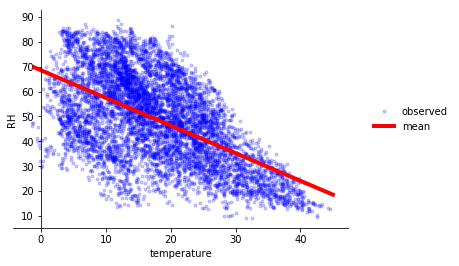
\includegraphics[width=0.7\textwidth]{./figs/no_unc_rh.png}
    \caption{Prognose der relativen Luftfeuchtigkeit}
    \label{fig:no_unc_rh}
\end{figure}

\begin{figure}[h]
    \centering
    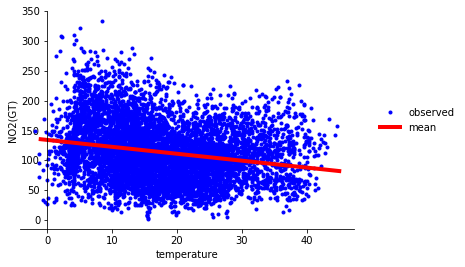
\includegraphics[width=0.7\textwidth]{./figs/no_unc_no2.png}
    \caption{Prognose des Stickstoffgehalts in der Luft}
    \label{fig:no_unc_no2}
\end{figure}


\subsubsection{Modellierung mit Unsicherheit}
\label{sec:with_unc}

Betrachtet man sich Abbildung \ref{fig:no_unc_rh} fällt auf, dass die Unsicherheit des hier linearen Ansatzes bei geringen Temperaturen stark zunimmt. Mit anderen Worten: Die Genauigkeit lässt nach. Das Modell kann dieses Problem aber noch nicht repräsentieren, daher wird im folgenden, verbesserten Modell die Unsicherheit integriert. Listing \ref{lst:model_with_uncertainty} beschreibt die Änderung. Der Aufbau ist dem ersten sehr ähnlich und unterscheidet sich im Wesentlichen nur in zwei Aspekten: 

\begin{itemize}
  \item Die erste Schicht hat einen zweidimensionalen Ausgabevektor, um die Unsicherheit mit darzustellen.
  \item Die zweite Schicht verwenden den zweiten Wert des Vektors, um seine Standardabweichung zu definieren. 
\end{itemize}

\begin{lstlisting}[language=Python, caption={Modell mit Keras mit Unsicherheit}, label={lst:model_with_uncertainty}]
def model_with_uncertainty(feature, label, epochs=5000):
  # feature
  x = np.array(df[feature])
  x = x[..., np.newaxis]

  # label
  y = np.array(df[label])
  
  model = tf.keras.Sequential([
    tf.keras.layers.Dense(2),
    tfp.layers.DistributionLambda(lambda t: tfd.Normal(
        loc=t[..., :1],
        scale=1e-3 + tf.math.softplus(5e-3 * t[...,1:])))
  ])

  # inference
  negloglik = lambda y_, rv_y: -rv_y.log_prob(y_)
  model.compile(optimizer=tf.compat.v2.optimizers.Adam(learning_rate=0.01), loss=negloglik)
  model.fit(x, y, epochs=epochs);

  return (x, y, model)
\end{lstlisting}

Das Ergebnis lässt sich in den Abbildungen \ref{fig:with_unc_rh} und \ref{fig:with_unc_no2} ablesen. Die Standardabweichung ist nun Teil des Modells. Akzeptiert man hier das lineare Modell, lässt sich für den Stickstoffgehalt in der Luft allgemein aussagen, dass die Prognosesicherheit mit steigenden Temperaturen sinkt und der Stickstoffgehalt in Luft interessanter Weise ebenfalls fällt. Am Modell der relativen Luftfeuchtigkeit  lässt sich durch das probabilistische Modell ablesen, dass bei steigenden Temperaturen die Genauigkeit der Prognosen stark zunimmt, was sich mit der Erwartungshaltung gegenüber der Relation von Temperatur und Luftfeuchtigkeit deckt.

Auffällig ist hier, dass die Prognose der Unsicherheit des Stickstoffgehalts die Daten nicht sehr genau abbildet. Das kann mehrere Gründe haben. Hier wurde nur ein einfaches lineares Modell für Demonstrationszwecke verwendet. Einige der Hyperparameter könnten weiter angepasst werden und die Trainingszeit oder Datenmenge ist nicht unbedingt ausreichend. Natürlich kann es auch sein, dass die Temperatur kein sinnvoller Maßstab für den Stickstoffgehalt in der Luft ist, wodurch das Modell keine große Aussagekraft besitzt. 

\begin{figure}[h]
    \centering
    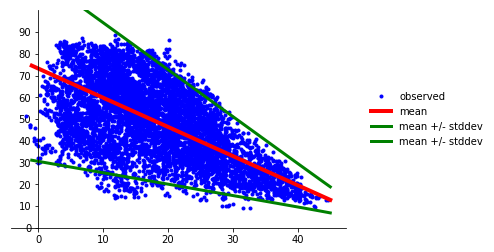
\includegraphics[width=0.7\textwidth]{./figs/with_unc_rh.png}
    \caption{Prognose der relativen Luftfeuchtigkeit mit variabler Standardabweichung}
    \label{fig:with_unc_rh}
\end{figure}

\begin{figure}[h]
    \centering
    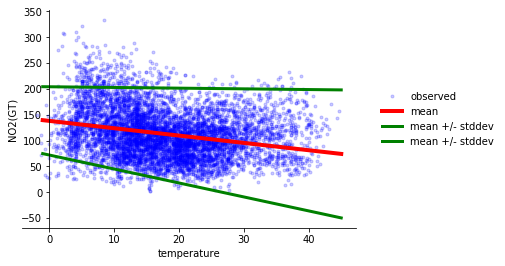
\includegraphics[width=0.7\textwidth]{./figs/with_unc_no2.png}
    \caption{Prognose des Stickstoffgehalts in der Luft mit variabler Standardabweichung}
    \label{fig:with_unc_no2}
\end{figure}


\section{Fazit}

Die Bibliothek TFP ist eine praktische Erweiterung des Tensorflow Frameworks, um sein Modell um eine probabilistische Ebene zu erweitern. Die bereitgestellten Funktionen sind sinnvoll aufgeteilt und es sind im Normalfall Beispiele für deren Verwendung vorhanden. Auch beim Release von Tensorflow 2.0 wurden Anpassungen an TFP vorgenommen, was das Interesse von Google und der OpenSource Community an der Weiterentwicklung von TFP zeigt. 

Die Einarbeitungszeit ist, auch unter Ansicht der Komplexität des Themengebietes, nicht zu Vernachlässigen. Ein Beispiel hiervon sind \textit{Dataflow Graphs}. \textit{Dataflow Graphs} von Tensorflow ermöglichen ein effizientes Berechnungsmodell, welches auf GPUs und auf neuere spezialisierte Hardware wie TPUs ausgelegt ist. Einfache Anwendungsfälle profitieren aber nicht unbedingt von der Abstraktionsebene von Tensorflow. Eine alternative und bekannte Bibliothek für probabilistische Programmierung in Python, anstelle von TFP, ist beispielsweise \textit{PyMC3}\footnote{\url{https://docs.pymc.io/}}.

Besonders im Hinblick auf maschinelles Lernen eignet sich der Einsatz von TFP. Es reiht sich relativ problemlos in das bestehende Framework ein. Die Integration in Keras ist einer der nennenswertesten Stärken von TFP, da die Komplexität an der richtigen Stelle gelockert wird. Probabilistische Modelle zu Erstellen wird hierdurch nicht trivial, aber deutlich zugänglicher. Ein fundamentales Wissen über die Domäne und das breite Gebiet der der Wahrscheinlichkeitstheorie ist natürlich immer noch erforderlich. 

\section{Materialien}

An dieser Stelle möchte ich eine Auswahl an hilfreichen Materialien zum Thema \textit{bayesian programming} aufführen, welche mir bei der Recherche positiv aufgefallen sind:
\begin{itemize}
  \item Jährliche Konferenz über Baysian Deep Learning (NIPS) \url{http://bayesiandeeplearning.org/}
  \item Machine Learining: A Probabilistic Perspective (Kevin P. Murphy)\cite{Murphy2012}
  \item Präsentation über Tensorflow Probability des Entwicklers Josh Dillon \url{https://youtu.be/GqxmRKplj4w} (Folien: \url{https://docs.google.com/presentation/d/1BWhNVHzhFfYiFL8ynX1wFmag8YjzvHeqKkd8Z0G8H7Y/edit#slide=id.g3f2acb32c4_0_0})
\end{itemize}


%----------------------------------------------------------------------------------------
%	Bibliography
%----------------------------------------------------------------------------------------
\newpage

\typeout{===== Section: literature}
\bibliography{bibs/bibs}

\listoffigures
\lstlistoflistings

\end{document}


